\documentclass[11pt]{article}
\usepackage[letterpaper,margin=1in]{geometry}
\usepackage{color}
\usepackage[dvipdfmx]{graphicx}
\usepackage{amsbsy}
\usepackage{amsmath}
\usepackage{adjustbox}
\usepackage{url}
%\usepackage{floatrow}
\usepackage[font=small,labelfont=bf,tableposition=top]{caption}
\DeclareCaptionLabelFormat{tableonly}{\tablename~\thetable}
%\newfloatcommand{capbtabbox}{table}[][\FBwidth]


\newcommand{\argmax}{\mathop{\rm arg~max}\limits}

\begin{document}
\vspace{-1cm}
%\title{\vspace{-2ex}Analysis Report on Assignment 3: SVM\vspace{-2ex}}
\title{Analysis Report on Assignment 3: SVM}
\author{Yoshinari Fujinuma\vspace{-2ex}}
\date{\vspace{-2ex}}
\maketitle

For the rest of the analysis, the ratio of the training data size to the test data size of the SVM model is $8:2$. 
In general, the larger the $C$ is, the smaller the margin becomes.
According to Figure \ref{linear_kernel}, the larger the $C$ becomes, the better the held out accuracy becomes for the RBF kernel.
This is because the RBF kernel has more expressive power than the linear kernel so the smaller margin helps the RBF kernel overfitting to the training data. Therefore, the smaller the margin is, the better the classification accuracy becomes.
For the linear kernel, the larger the $C$ becomes, the held accuracy becomes slightly worse as shown in Figure \ref{rbf_kernel}. This shows that the decision boundary does not differ much by how large the margin is for the linear kernel.

\begin{figure}[htb]
  %\vspace{-1.1cm}
  \begin{center}
   \begin{tabular}{c}
    \begin{minipage}{0.5\hsize}
     %\vspace{-0.5cm}
     \begin{center}
     %\scalebox{0.25}
     \scalebox{0.33}
      {\includegraphics[]{figure_4_C.png}}
   
      \caption{\label{linear_kernel}Different C values for SVM with the linear kernel.}
      \label{fig:learning_rate}
     \end{center}
    \end{minipage}

    \begin{minipage}{0.01\hsize}
    \end{minipage}

    \begin{minipage}{0.5\hsize}
     \begin{center}
      \scalebox{0.33}
      {\includegraphics[]{figure_3_C.png}}
      \caption{\label{rbf_kernel}Different C values for SVM with the RBF kernel.}
     \end{center}
    \end{minipage}

  \end{tabular}
 \end{center}
\vspace{-0.5cm}
\end{figure}




\begin{figure}[htb]
  %\vspace{-1.1cm}
  \begin{center}
   \begin{tabular}{c}
    \begin{minipage}{0.5\hsize}
     %\vspace{-0.5cm}
     \begin{center}
     %\scalebox{0.25}
     \scalebox{0.33}
      {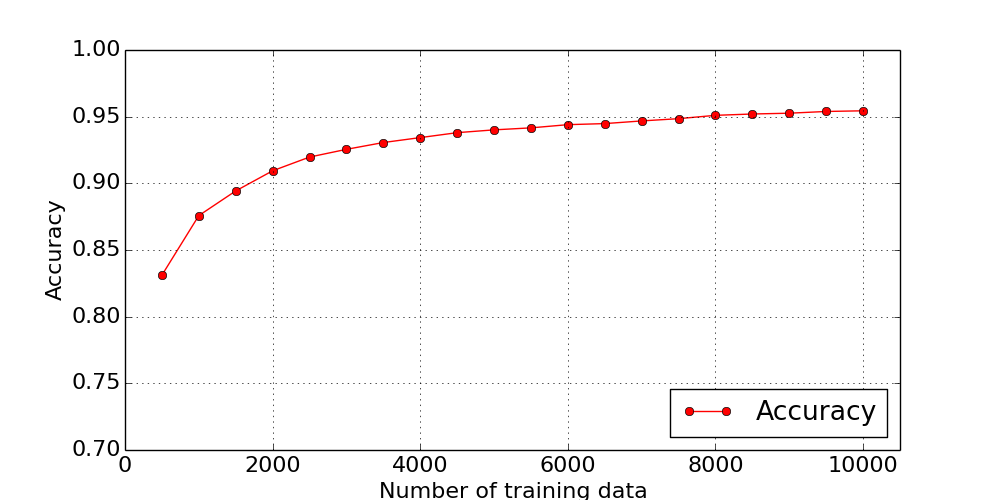
\includegraphics[]{figure_1.png}}
   
      \caption{The support vector for class $3$. }
      \label{fig:support_vector_1}
     \end{center}
    \end{minipage}

    \begin{minipage}{0.01\hsize}
    \end{minipage}

    \begin{minipage}{0.5\hsize}
     \begin{center}
      \scalebox{0.33}
      {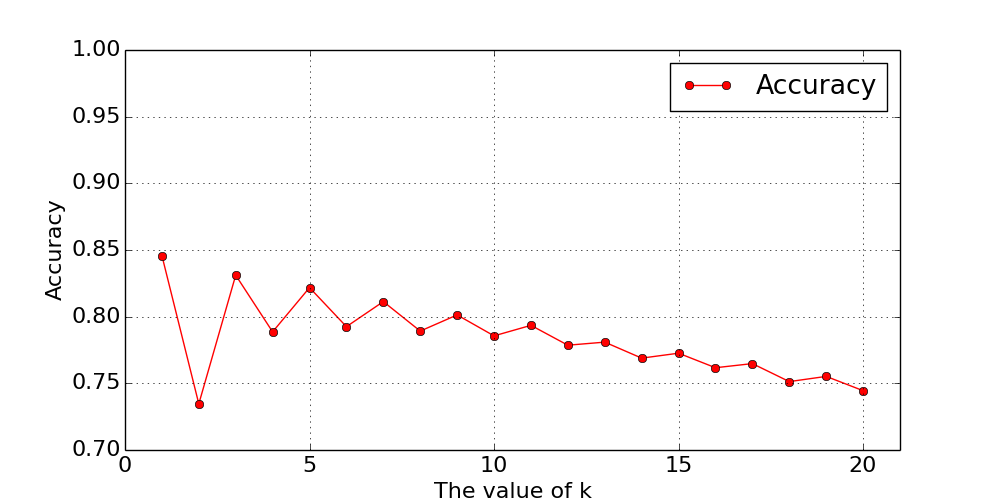
\includegraphics[]{figure_2.png}}
      \caption{\label{fig:support_vector_2}The support vector for class $8$.}
     \end{center}
    \end{minipage}

  \end{tabular}
 \end{center}
\vspace{-0.5cm}
\end{figure}

Examples of the support vectors from the linear kernel are shown in Figure \ref{fig:support_vector_1} and Figure \ref{fig:support_vector_2}. The support vectors do catch difficult examples. In Figure \ref{fig:support_vector_1}, the support vector for $3$ does lack the bottom stroke. The support vector for the label $8$ in Figure \ref{fig:support_vector_2} have only two very narrow circles which makes the structure close to $3$.


\end{document}
